\chapter{Conclusion}

\section{Results}

\section{Limitations}

Throughout this research Dynamic OpenCL was proven to efficiently compute a variety of algorithms and  execute a multitude of jobs in parallel through a two tiered scheduling infrastructure. Still, in its current version it suffers from several factors that either limit its performance or general functionality.

For instance, while Dynamic OpenCL is deeply rooted to Aparapi and profits from its compelling features it is also limited by it in the complexity of writable code. As explained in section \ref{aparapi} not every Java code can be translated to OpenCL by Aparapi and the respective capabilities of Dynamic OpenCL are therefore tied to Aparapi.

While Dynamic OpenCL is able to operate heterogeneous clusters with different hardware vendors and device types, the varying feature sets of devices may become problematic for certain workloads. In section \ref{opencl} an example about the \textit{FP64} feature was portrayed that might be missing for some devices within a cluster. Dynamic OpenCL is currently not able to identify these features and can therefore not schedule appropriately. This means that workloads with a requirement for a specific feature may be assigned to nonsupporting devices and thus produce an error.

During this research Dynamic OpenCL was run for many different cluster compositions and workloads. It is concluded that the network bandwidth is the major limiting performance factor. While this bottleneck is identifiable by the benchmarks run during the evaluation another hardware limitation exists that is caused by the architecture of Dynamic OpenCL. In the general setup a central node exists that manages all running tasks within a cluster. Throughout the execution of a job it has to hold on to the input data while it also receives partial results from the compute nodes. This data has to be kept in memory and in the case of multiple data intense jobs can fill the entire RAM. In an appropriate cluster setup the central node therefore holds sufficient RAM to support expected peaks in parallel running jobs. Another strategy is to block further job submissions once memory reaches its maximum utilization.

jobs that make sense


\section{Future Work}

In its current state Dynamic OpenCL is a research prototype and as such still requires significant improvements concerning stability. Additionally, certain features that tackle the previously described limitations of the framework are desirable in the future. While there are numerous potential improvements to the framework, this section covers more substantial topics that can greatly enhance the performance and usability of Dynamic OpenCL.

\subsection{Workload Queuing}

As shown by the evaluation the overall performance of Dynamic OpenCL is heavily dependent on the available networking capabilities within the cluster. In the current version there might be periods were data transfers to different machines overlap, thus competing for bandwidth. At the same time when all devices in the cluster are computing, no data transfers are processed. A possibility to improve execution speed of the system is to reduce idle times of the network and instead use the unused bandwidth to transfer data for future tasks.

\begin{figure}[H]	
	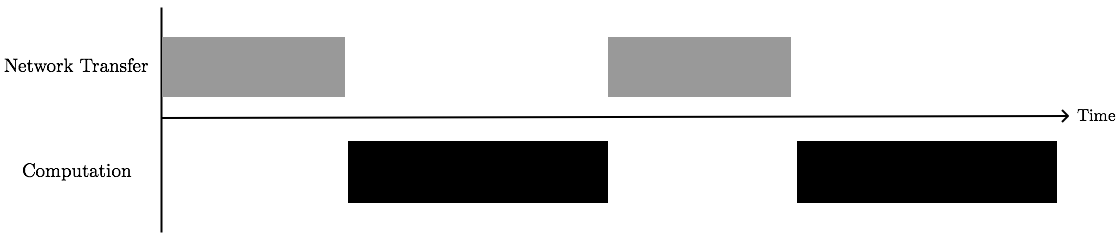
\includegraphics[width=0.85\textwidth]{images/missing_queuing.png}
	\centering
	\caption{Current Execution Workflow}
	\label{img:missing_queuing}
\end{figure}

\subsection{Cloud Cost Optimization}

\section{Final Thoughts}
